
Chapter 2 goes here ...


%----------------------------------------------------------------------
\section{First Section} 
\label{sec:SECTION1NAME}

 
Secure multi party protocols among non trusting parties have been
developed and found applications in various areas (privacy preserving 
distributed data mining, secure computational geometry, etc...). However such
secured protocols in a multi robotic or distributed robotic framework have
been rare or perhaps non existent. In one such initial attempt we try to
apply principles of secure multi party computation to a multi-robotic
framework to solve what we feel is a practical problem.

\begin{figure}
\centering
\subfloat[Initial Positions]{\label{fig:1a}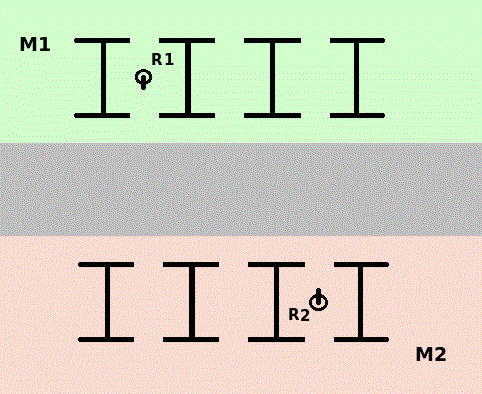
\includegraphics[width=0.3\textwidth]{figure-1a.png}}
\hspace{10pt}
\subfloat[Hypotheses as point clusters]{\label{fig:1b}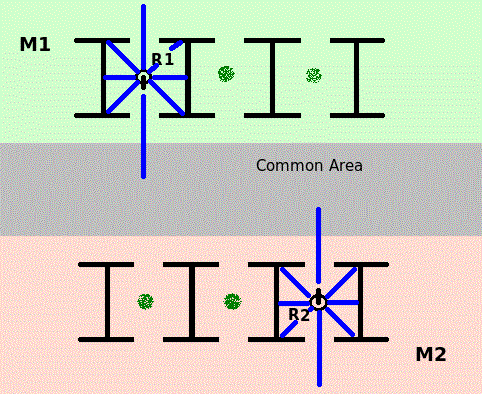
\includegraphics[width=0.3\textwidth]{figures/fig-1b.png}}
\caption{Localization of multiple robots}
\label{fig:1}
\vspace{-20pt}
\end{figure}


Figure 1a shows a robot R1 in its map M1 and robot R2 in its map M2 both
unaware of their positions represented by the tuple   in their maps. The
robots possess a compass by which they obtain their orientation. In order
to estimate their positions they perform global localization based on a
Markov framework~\cite{Fox98:M}. This results in multiple
hypotheses states for both R1 and R2, in this case three each (Fig 1b). In
previous approaches~\cite{BKG07,BK08} we have shown how robots can help each other
to localize to a unique state by moving to places where they can obtain
unique measurements between them that is not possible from anywhere else
in the environment. This inevitably requires exchange of map information.
In this paper we show how amongst non-trusting robots the same outcome is
achieved (robots get localized to a unique state) without the robots ever
getting in possession of the others map. This is achieved through a secured 
multiparty computation of the localization algorithm, where each robot shares 
its map in such a way that the other robot cannot gain any information about it.

In futuristic scenarios where several robots will operate together it is
difficult to expect that the robots would exchange all their information
between each other. For example robots belonging different agencies/
companies may operate in a floor of a building. They may for reasons of
security not want to share information, however they may need to perform
tasks together that involves such transfer of information. The problem
being attacked in this paper is one such example where non-trusting agents
need to cooperate to achieve their goals.

%
%This is to insert a table \\
%
%\begin{table}
%\begin{center}
%\begin{tabular}{|l|c|}
%\hline
%Method & Frobnability \\
%\hline\hline
%Theirs & Frumpy \\
%Yours & Frobbly \\
%Ours & Makes one's heart Frob\\
%\hline
%\end{tabular}
%\end{center}
%\caption{Results.   Ours is better.}
%\end{table}
%

%----------------------------------------------------------------------

\section{Secure Multiparty Computation}
\label{sec:smpc}

Imagine a situation where several parties wish to achieve a common goal, but they do not trust
each other to reveal their private information. Examples of such situations are abundant in the
real world, such as distributed voting, private bidding and auctions, and privacy preserving data 
mining. One naive strategy is to find a trusted third party, give that third 
party all the inputs, and ask him to publish the answer. Finding such a third party is usually
difficult, if not impossible. One also has to ensure that such a third party cannot violate 
or abuse the information sent to him, or else the strategy is defeated.

Secure Multiparty Computation~\cite{GMW87:HtPaMG} deals with answering the following:
given there are $n$ parties each with their inputs $\iota_{n}$, how to evaluate a function 
$f(\iota_{1},...,\iota_{n})$ operating on these inputs, such that no party $j$ gets to know 
the input of party $k$, $\forall j \neq k$. 

In an ideal world, a trusted third party (TTP) can be found. All the players can then
send their information to the TTP, the TTP processes the information recieved, and sends back the 
respective results to the players. Since in the real world finding such a TTP is difficult, SMPC protocols 
ensure a way to simulate the ideal world TTP among the players themselves~\cite{GMW87:HtPaMG}. Whatever operations 
an ideal world TTP performs, each of them is simulated among the players in the real world. In the 
ideal world, since privacy and correctness are ensured automatically, and since those same operations
are simulated in the real world, one can rest assured that the real world executions also ensure
privacy and correctness.

\section{Tools and Techniques}
\label{sec:tt}

We now present here methods to securely compute addition, multiplication, set union
and maximisation. The methods presented here for addition and multiplication
are secure in the sense that no information other than the results is revealed. Most 
Secure Multiparty Protocols are carried out in two phases: the sharing phase and the 
reconstruction phase. In the sharing phase, a secret is shared among all the players in such
a way that no information about the secret is revealed. If $\mathcal{P}$ is the set of players
who wish to compute the actual value of the secret, then the players in $\mathcal{P}$
need to execute the reconstruction phase. All the players who execute the reconstruction 
phase will know the secret. 

A $(k,n)$ secret sharing scheme~\cite{S79:HtSaS} is a scheme no information can be extracted by any $k$ players,
but can be reconstructed by any set of $k+1$ players. Here, since we assume that there are no 
collusions among robots, (that is, there are only robots, no robot teams) we can set $k = 1$. 
To tolerate any collusions of size $k$, we would need a k-degree polynomial, and hence here we 
use a straight line.


\begin{algorithm}
\caption{On sharing a secret}
\label{algshare}
\begin{algorithmic}
\REQUIRE A player has a secret value $v$ which he has to share
\STATE select a random number $r$
\STATE $f(x) = v + rx$
\FOR{all players $i$}
	\STATE send the value $v_{i}= f(i) = v + r(i)$ to player $i$
\ENDFOR
\ENSURE each player has a share $v_{i}$ of the secret $v$
\end{algorithmic}
\end{algorithm}

\begin{algorithm}
\caption{On reconstructing a secret}
\label{algrecon}
\begin{algorithmic}
\REQUIRE Each player has a share $v_{i}$ of the secret.
	$\mathcal{P}$ is the set of players who wish to reconstruct the secret.
\FOR{all players $i$}
	\STATE all the players send their shares to players in $\mathcal{P}$
\ENDFOR
\FOR{all players in $\mathcal{P}$}
	\STATE construct a polynomial $f(x) = a + bx$ which passes through all the points $(i,v_{i})$
	\STATE return the secret $v = a$
\ENDFOR
\ENSURE each player knows the secret $v$
\end{algorithmic}
\end{algorithm}

Notice that each player can know nothing about the secret as long as he knows only his share, $v_{i}$.
This ensures privacy of the secret. After the algorithm has completed, the secret answer is known only during
reconstruction, where all the players in $\mathcal{P}$ participate, and hence the answer is reconstructed.


\subsection{Secure Addition}
\label{sec:add}
Suppose there are $n$ players, holding secret values $s_{1}, ..., s_{n}$, and wish to compute
the sum, $s = \sum_{i = 1}^{n}s_{i}$. Each player simply shares his secret. Now that each player 
has recieved shares of every other player, he computes the sum of the shares. The new shares are
shares of the actual answer, the sum. This holds, because if $f_{s}(x) = \sum_{i = 1}^{n}f_{s_{i}}(x)$,
and the constants of the $f_{s_{i}}(x)$ polynomial are the secrets $s_{i}$, then the constant term
of the polynomial $f_{s}(x)$ is $\sum_{i = 1}^{n}s_{i}$, the required answer.


\begin{algorithm}
\caption{Computing Secure Addition}
\label{algadd}
\begin{algorithmic}
\REQUIRE $n$ is the number of players, each with private input $s_{i}$.
\STATE \COMMENT{Phase 1: Sharing}
\FOR{each player $i$}
	\STATE Share secret $s_{i}$
	\FOR{each player $j$}
		\STATE send $j$'s share $s_{ij}$ to player $j$
	\ENDFOR
\ENDFOR
\FOR{each player $j$}
	\STATE $sum_{j} = \sum_{i=1}^{n}s_{ij} $
\ENDFOR
\end{algorithmic}
\end{algorithm}

Now that each player has a share of the sum, if the players wish to publicly reveal the secret, 
they use the reconstruction algorithm given in protocol~\ref{algrecon} on their shares.


\subsection{Secure Multiplication}
\label{sec:mult}

For multiplication, we have a protocol given by~\cite{GRR98:SVFMCwAtTC}, which takes multiple rounds of communication, and 
is a little complex. Here, we present a simple and elegant protocol, with an initial preprocessing stage. The
preprocessing uses the protocol of~\cite{GRR98:SVFMCwAtTC}, but only once. All subsequent multiplications can be executed, using
the protocol~\ref{algmult}. The advantage with this protocol is that there is lesser communication complexity, 
and the computation can be done on the local shares.

We look at the simpler case of multiplying two secrets, $\alpha$ and $\beta$, 
which are assumed to be already shared among the $n$ players. In the initial preprocessing stage, 
we share two random numbers $x$ and $y$, and their product $xy$, while keeping the values themselves secret. 
The protocol given in ~\cite{GRR98:SVFMCwAtTC} is used to calculate $xy$. 

The numbers $\alpha$, $\beta$, $x$, $y$, $xy$ are now shared among the players. Now each player $i$ computes the values 
$\lambda_{i} =  \alpha_{i} - x_{i}$ and $\lambda_{i}' = \beta_{i} - y_{i}$, where $\eta_{i}$ stands
for the player $i$'s share of the value of $\eta$. Now the values of $\lambda$ and $\lambda'$ are 
reconstructed, that is, made public among the players. This affords no information gain about the values
of $\alpha$ and $\beta$, as $x$ and $y$ are still private. 
%One can easily verify that $\alpha\beta = \lambda\lambda' + y\lambda + x\lambda' + xy$ where $\lambda = \alpha -x$ and $\lambda' = \beta - y$.

Due to the linearity of the secret sharing protocol, we know that $\lambda = \alpha - x$ and $\lambda' = \beta - y$.
Also, 
\begin{eqnarray*}	
	\alpha\beta 	& = & (\alpha - x + x)(\beta - y + y) \\
			& = & (\alpha - x)(\beta - y) + y(\alpha - x) + x(\beta - y) + xy \\
			& = & \lambda\lambda' + y\lambda + x\lambda' + xy
\end{eqnarray*}

Since the respective shares of $x$, $y$ and $xy$ are already with the players, the computation of $\alpha\beta$
(rather the computation of the \emph{shares} of $\alpha\beta$) can be done locally. Since all the players have the shares of
the product, the required product can be reconstructed easily. This minimizes the cost of repeated multiplication,
which is very communication expensive. Also, the shares of $x$ and $y$ can be reused for all further multiplications,
without any loss of information.

\begin{algorithm}
\caption{Computing Secure Multiplication}
\label{algmult}
\begin{algorithmic}
\REQUIRE All the players have shares of random numbers $x$ and $y$ and their product $xy$.
They also have shares of $\alpha$ and $\beta$, of which they need to evaluate the product.
\STATE \COMMENT{Phase 1: SHARING}
\FOR{player $i$}
	\STATE  $\lambda_{i} = \alpha_{i} - x_{i}$
	\STATE $\lambda_{i}' = \beta_{i} - y_{i}$
	\STATE reconstruct the values $\lambda$ and $\lambda'$
	\STATE $\alpha\beta_{i} = \lambda\lambda' + y_{i}\lambda + x_{i}\lambda' + xy_{i}$
\ENDFOR
\end{algorithmic}
\end{algorithm}


\subsection{Secure Union}
\label{sec:onion}

Owing to the protocols given above for secure addition and multiplication, we can rest assured that 
any algebraic function can be evaluated securely, since every function is but a series of repeated parametric
additions and multiplications, and their inverses (subtractions and divisions). Also, assuming that every player
can locally generate a random number, we can also safely say that every probabilistic polynomial time algorithm
can be executed securely by the players. Formal proofs of these claims exist in literature, but they are out of 
the scope of this paper. However, in addition to these protocols, we also present some specific purpose protocols
such as this one for Secure Union.

Let every player $i$ have a private set $S_{i}$, where $S_{i} \subset {S}$ is the universal set, of size $k$.
Without loss of generality, we assume that the set ${S}$ is ordered, and that ${s_{i}| 1 \leq i \leq k}$ are 
the elements. Each player creates a binary array, $A_{i} = [a_{ij}]$, where $a_{ij} = 1$ if $s_{j} \in S_{i}$ and $0$ otherwise.
Now it remains to logically OR the arrays $A_{i}$ bitwise, and create the union set $U$. Note that, in binary operations, 
the AND gate corresponds to multiplication, and the XOR gate corresponds to addition. We have already described protocols
for multiplication and addition. The only difference here will be that the coefficients, operands and operations are in 
binary logic. Also, the OR gate can be decomposed to the AND and XOR gate. And since we know the protocols for these
gates, the OR gate can also be computed. The algorithm for the construction of secure union set is given below.

\begin{algorithm}
\caption{Constructing Secure Union}
\label{algonion}
\begin{algorithmic}
\REQUIRE player $i$ has the array $A_{i} = [a_{ij}]$ which represents the set $S_{i}$
\FOR{bit $j$ from $j = 1$ to $k$}
	\FOR {all players}
		\STATE share bit $a_{ij}$ in binary \COMMENT{Use the protocol~\ref{algadd}}
		\STATE construct bit $XORa_{j} = {XOR}_{t=1}^{n}a_{ij}$ using protocol~\ref{algadd}
		\STATE construct bit $ANDa_{j} = {AND}_{t=1}^{n}a_{ij}$ using protocol~\ref{algmult}
		\STATE construct bit $ORa_{j} = XORa_{j} XOR ANDa_{j}$ using protocol~\ref{algadd}
		\STATE element $u_{j} = ORa_{j}$
	\ENDFOR
\ENDFOR
\STATE return set $U = \{u_{j}|j = 1 $ to $ k\}$
\end{algorithmic}

\end{algorithm}

The protocol for secure intersection is similar to this, where instead of constructing the XOR of the 
bits, just an AND of the bits is enough. Which is to say that a modified multiplication protocol will 
be the same as a secure intersection protocol. 


\subsection{Secure Maximisation}
\label{sec:max}

We suppose that the $n$ players each have a private input value, a probability, in the range $[0,1]$, and that
they wish to find out the maximum value amongst them, and the player who holds it. The protocol mimics the binary 
search over a given range. First, the interval is divided into two halves, $[0,0.5]$ and $[0.5,1]$, and the number of
players in the greater interval are counted. Then, the interval with the largest value is subdivided into two halves,
and the same process is repeated recursively, until only one player remains in the greater interval. This 
value is then shared.

\begin{algorithm}
\caption{Maximisation of probabilities}
\label{algmax}
\begin{algorithmic}
\REQUIRE each player has a private value $p_{i}$ within the range $[0,1]$
\STATE $A = 0, B = 1$
\LOOP
\STATE $C = (A + B) / 2$
\FOR{each player $i$}
	\STATE $a_{i} = 0 $; $b_{i} = 0$
	\IF{value $p_{i} < C$ }
		\STATE $a_{i} = 1 $
	\ELSE
		\STATE $ b_{i} = 1$
	\ENDIF
	\STATE \COMMENT{Use the Secure Addition protocol~\ref{algadd}}
	\STATE add all players' private $a_{i}$'s and $b_{i}$'s, call them $a$ and $b$
	\STATE reconstruct $a$ and $b$
	\IF{$b \geq 1$}
		\STATE $A = C$ and continue loop
	\ELSIF{$b = 1$}
		\STATE exit loop \COMMENT{Player with max value found}
	\ELSIF{$a \geq 1$}
		\STATE $B = C$ and continue loop
	\ELSE
		\STATE exit loop \COMMENT{Player with max value found}
	\ENDIF
\ENDFOR
\ENDLOOP
\STATE \COMMENT{All players know for themselves whether they are or not the one with the max value}
\FOR{all players $i$}
	\IF{$a_{i} = 1$ or $b_{i} = 1$}
		\STATE share value $p_{i}$
	\ELSE
		\STATE share $0$
	\ENDIF
\ENDFOR
\end{algorithmic}
\end{algorithm}



All the above mentioned algorithms and protocols end with the actual answer being shared. 
For the answer to be revealed, one can always run the reconstruction algorithm (protocol~\ref{algrecon}).

\section{Secure Active Localization}
\label{sec:secloc}

Armed with the above primitives, we can now construct the algorithm for securely localizing the multiple robots.
Each robot knows a part ($M_{i}$) of the global map($GM$), which it does not wish to reveal. None of the robots know
the global map, but they are curious to find out whatever they can about it. Also, parts of the map $M_{i}$ are 
symmetric, and hence the robots are in confusion regarding their initial position. They can actively localize according 
to the existing algorith, but for that they will have to reveal their private maps. The secure multiparty protocols
provide a way out, in the sense that, they allow the execution of the localization algorithm, without the players 
having to reveal their private maps.

The robots do not trust each other, and they do not team up or share information within themselves. That is, there are
no collusions or cliques among the players. But since the localization algorithm has to be executed, 
each robot does not reveal its map, but instead creates a multiparty share of the map. Without reconstructing the global 
map, (since none of the robots want to reveal their private maps) the localization algorithm is run on the shares of the 
global map. The resulting combinations are reconstructed, since each robot needs to know which frontier it should move to. 

Also, since the protocols guarantee that the individual shares are never revealed at the end of the computation, the 
private maps are never revealed. The algorithm is run on the share of the global map. For every addition step in the 
algorithm, the local shares are added. For every multiplication step, the preprocessed shares of $x$, $y$ and $xy$ are used, 
the computation is done locally as shown, and the result is 
reconstructed publicly. At the end of all these steps, finally the algorithm results in the shares of a combination, 
rather a robot to frontier mapping. A reconstruction of this mapping results in each robot being told a frontier to move to. 



\begin{algorithm}
\caption{Secure Active Localization}
\label{algsecloc}
\begin{algorithmic}
\STATE \COMMENT{All addition operations are addition of local shares}
\STATE \COMMENT{All multiplication operations follow the protocol\ref{algmult}}
\REQUIRE Each player has a private map $M_{i}$
\FOR{all robots $i$}
\STATE share private map $M_{i}$ using the protocol~\ref{algshare} \COMMENT{step 1}
\STATE \COMMENT{ $M_{ji}$ is $i$'s share of $j$'s private map }
\STATE construct share of global map $GM_{i} = \cup_{j=1}^{n}M_{ji}$
\STATE \COMMENT{Union is constructed using protocol~\ref{algonion}}
\ENDFOR
\REPEAT
\STATE go to the frontier last specified
\STATE take sensor readings
\STATE share sensor readings using protocol~\ref{algshare}
\STATE create hypotheses
\STATE share hypotheses	\COMMENT{step 2}
\IF{\# of Hypotheses = 1}
\STATE localized = TRUE
\ENDIF
\IF{localized = TRUE}
	\IF{another robot is visible}
		\STATE update the other robot's belief
	\ENDIF
\ENDIF
\STATE calculate possible frontiers
\STATE share the set of frontiers
\FOR{each robot $i$}
	\FOR{each frontier}
		\STATE calculate occupancy probability of this frontier by the robot $i$
	\ENDFOR
\ENDFOR
\STATE create all possible combinations of robots going to one of the frontiers
\FOR{all combinations c}
	\STATE calculate probability of Unique Measurement
\ENDFOR
\STATE Of all the combinations, select that which has maximum probability
\STATE reconstruct the combination, the frontier that each robot has to go to \COMMENT{step 3}
\UNTIL{all robots localize}
\end{algorithmic}
\end{algorithm}


\subsection{An Example}
\label{sec:ex}	

The method for active localization given in~\cite{BK08} is based on the assumption that all robots 
have knowledge of the full map. Here, we assume that each robot has only part of the global map, as
is shown in the figure~\ref{fig2a}. The robot R1 knows the map M1 and R2 knows M2, and so on. None of the robots 
wish to reveal its map to the other. There is a shared area, though, shaded in grey, which is known to all the robots.
The figure~\ref{fig2a} also shows the initial hypotheses that the robots have calculated, from their initial measurements.


The algorithm for the secure localization starts with each of the robots sharing its map, using 
protocol~\ref{algshare}, and sends the other robots each a share (step $1$ in algorithm~\ref{algsecloc}). 
The robots also share with each other
their list of hypotheses, in the same manner (step 2). Now each of the robot individually computes the active
localization alorithm of~\cite{BK08}, on these shares. Several subprotocols are run during this execution,
for several different operations, such as multiplication, union, and others described below. 
Ultimately, all the robots compute shares of the final frontiers that they ought to move, for a faster
localization. These shares are then given to the other players, so as to enable them to reconstruct
the final direction and frontiers they should move to (step 3). The directions and the final localized positions 
are shown in the figure~\ref{fig2b}. 

\begin{figure}
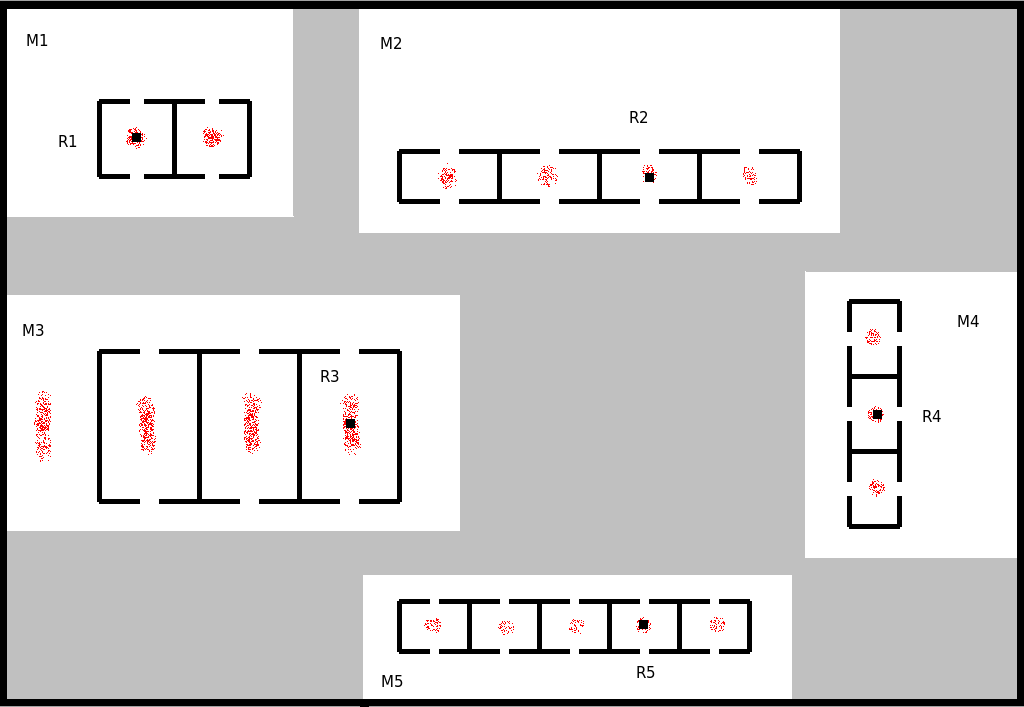
\includegraphics[width=\textwidth]{initial.png}
\caption{Initial Positions and Hypotheses}
\label{fig2a}
\end{figure}


Also, we assume that there are no collusions among the robots, that is, no robots are willing to trust 
any other robot, so they will not pool in information. The robots might be curious, though, and would want 
to extract whatever information they can about the other robots, from the execution of the algorithm. Since 
the SMPC protocols are based on co-operation among the robots, following the protocol correctly mutually 
helps all the robots. If one of the robots wishes to work against the protocol, then another robot might wish 
to work against the first. So if all the robots follow the protocol correctly, the execution is guaranteed to 
be correct. The methods to execute the algorithm even under such a scenario, and still guarantee 
the privacy of each player's input, are given in the next section.

\begin{figure}
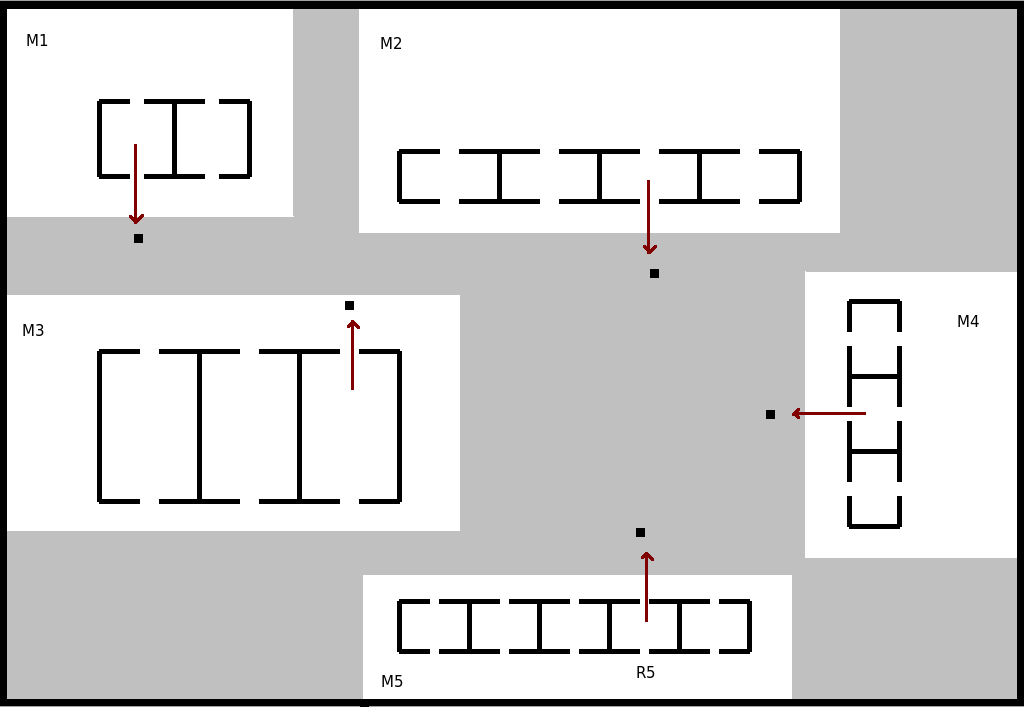
\includegraphics[width=\textwidth]{final.png}
\caption{Final localized positions}
\label{fig2b}
\end{figure}


